\documentclass[12pt,a4paper,oneside]{book}



\usepackage[utf8]{inputenc}

\usepackage[T1]{fontenc}

\usepackage{lmodern}

\usepackage{graphicx}

\usepackage{xcolor}

\usepackage{geometry}

\usepackage{tikz}

\usepackage{float}

\usepackage{tabularx}
\usepackage{array}
\usepackage{titlesec}
\usepackage{caption}
\usepackage{placeins}
\usepackage{listings}
\usepackage{chngcntr}

\usetikzlibrary{arrows.meta,shapes.geometric}



\geometry{margin=1in}
\raggedbottom
\setlength{\textfloatsep}{12pt plus 2pt minus 2pt}
\setlength{\floatsep}{10pt plus 2pt minus 2pt}
\setlength{\intextsep}{10pt plus 2pt minus 2pt}
\renewcommand{\topfraction}{0.90}
\renewcommand{\bottomfraction}{0.85}
\renewcommand{\textfraction}{0.10}
\renewcommand{\floatpagefraction}{0.75}

% Number code listings by section (for example, Code 27.3.1)
\AtBeginDocument{%
    \counterwithin{lstlisting}{section}%
    \renewcommand{\thelstlisting}{\thesection.\arabic{lstlisting}}%
}
\renewcommand{\lstlistingname}{Code}
\lstset{
    frame=single,
    rulecolor=\color{black},
    backgroundcolor=\color{gray!5},
    basicstyle=\ttfamily\small,
    numbers=left,
    numberstyle=\tiny\color{gray},
    numbersep=8pt,
    breaklines=true,
    breakatwhitespace=false,
    showstringspaces=false,
    keepspaces=true,
    columns=fullflexible,
    captionpos=b,
    xleftmargin=5pt,
    xrightmargin=5pt,
    aboveskip=12pt,
    belowskip=12pt
}

% Consistent report typography and numbered elements
\setcounter{secnumdepth}{3}
\setcounter{tocdepth}{3}
\renewcommand{\thesection}{\thechapter.\arabic{section}}
\renewcommand{\thesubsection}{\thesection.\arabic{subsection}}
\renewcommand{\thesubsubsection}{\thesubsection.\arabic{subsubsection}}
\renewcommand{\thefigure}{\thechapter.\arabic{figure}}
\renewcommand{\thetable}{\thechapter.\arabic{table}}
\captionsetup{font=small,labelfont=bf,justification=centering}
\captionsetup[table]{position=bottom}
\titleformat{\chapter}[display]
  {\normalfont\bfseries\Huge}{\chaptername\ \thechapter}{10pt}{\Huge}
\titleformat{\section}{\normalfont\Large\bfseries}{\thesection}{0.8em}{}
\titleformat{\subsection}{\normalfont\large\bfseries}{\thesubsection}{0.8em}{}

\begin{document}

\mainmatter



% Group 27 numbering: Chapter 27, sections 27.1, 27.2, subsections 27.1.1, etc.
\setcounter{chapter}{26}
\chapter{Employee Leave Management System (LeaveFlow)}



\section{System Architecture}



LeaveFlow follows a layered architecture consisting of a web

interface, a Flask application, a C++ processing component,

and local data storage. Flask manages authentication, role-based

access control, and leave records. It invokes the compiled C++

backend for leave validation and processing.



\begin{figure}[htbp]

\centering

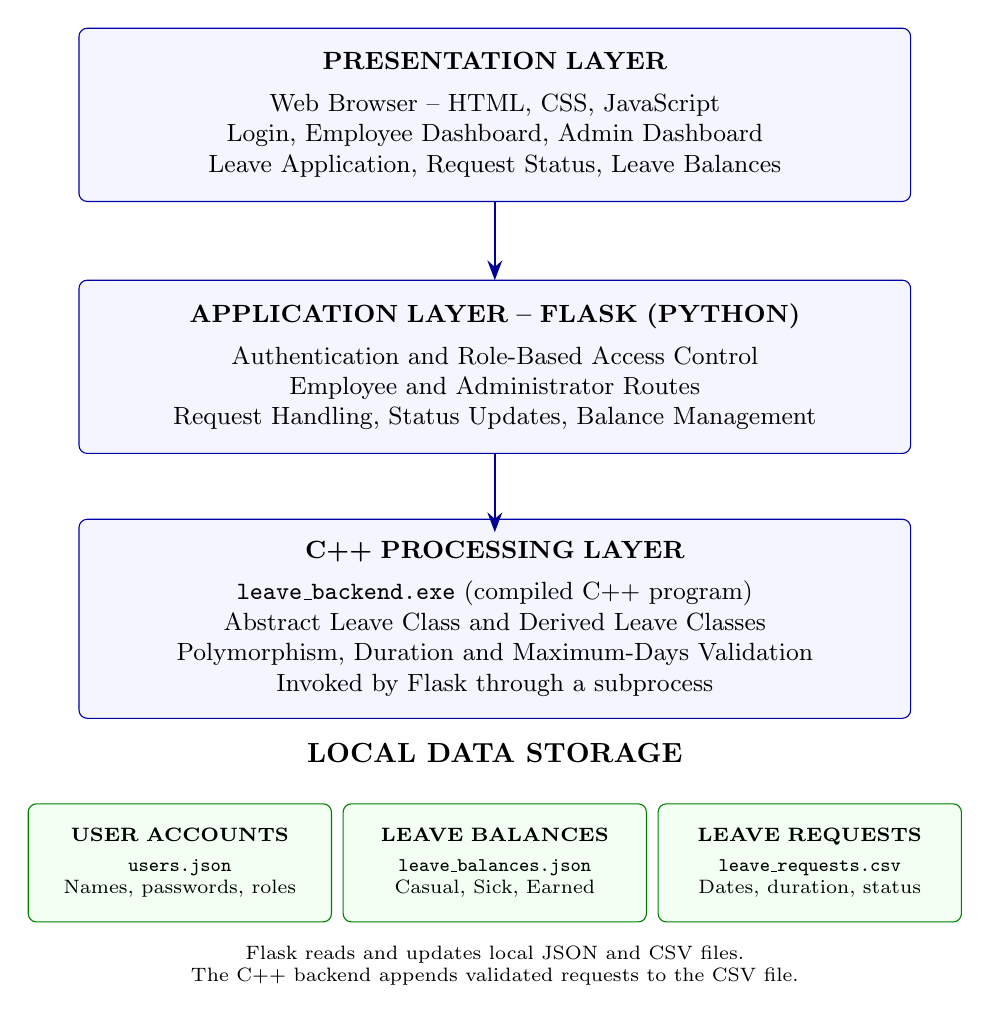
\begin{tikzpicture}[
    x=1cm,y=1cm,
    main/.style={
        draw=blue!65!black,
        fill=blue!4,
        rounded corners=3pt,
        align=center,
        text width=10cm,
        minimum height=2.2cm,
        inner sep=8pt,
        font=\small
    },
    storage/.style={
        draw=green!50!black,
        fill=green!5,
        rounded corners=3pt,
        align=center,
        text width=3.5cm,
        minimum height=1.5cm,
        inner sep=5pt,
        font=\scriptsize
    },
    flow/.style={
        -{Stealth[length=2.5mm]},
        thick,
        blue!60!black
    }
]
% Presentation layer
\node[main] (web) at (0,0) {
    \textbf{PRESENTATION LAYER}\\[4pt]
    Web Browser -- HTML, CSS, JavaScript\\
    Login, Employee Dashboard, Admin Dashboard\\
    Leave Application, Request Status, Leave Balances
};
% Flask layer
\node[main] (flask) at (0,-3.2) {
    \textbf{APPLICATION LAYER -- FLASK (PYTHON)}\\[4pt]
    Authentication and Role-Based Access Control\\
    Employee and Administrator Routes\\
    Request Handling, Status Updates, Balance Management
};
% C++ processing layer
\node[main] (cpp) at (0,-6.4) {
    \textbf{C++ PROCESSING LAYER}\\[4pt]
    \texttt{leave\_backend.exe} (compiled C++ program)\\
    Abstract Leave Class and Derived Leave Classes\\
    Polymorphism, Duration and Maximum-Days Validation\\
    Invoked by Flask through a subprocess
};
% Data storage heading
\node[font=\bfseries] at (0,-8.1) {
    LOCAL DATA STORAGE
};
% Data files
\node[storage] (users) at (-4.0,-9.5) {
    \textbf{USER ACCOUNTS}\\[3pt]
    \texttt{users.json}\\
    Names, passwords, roles
};
\node[storage] (balances) at (0,-9.5) {
    \textbf{LEAVE BALANCES}\\[3pt]
    \texttt{leave\_balances.json}\\
    Casual, Sick, Earned
};
\node[storage] (requests) at (4.0,-9.5) {
    \textbf{LEAVE REQUESTS}\\[3pt]
    \texttt{leave\_requests.csv}\\
    Dates, duration, status
};
% Simple vertical arrows
\draw[flow] (0,-1.1) -- (0,-2.1);
\draw[flow] (0,-4.3) -- (0,-5.3);
% Storage relationship description
\node[font=\scriptsize,align=center] at (0,-10.8) {
    Flask reads and updates local JSON and CSV files.\\
    The C++ backend appends validated requests to the CSV file.
};
\end{tikzpicture}



\caption{System architecture of the LeaveFlow application}

\label{fig:system-architecture}

\end{figure}



\section{Technology Stack}

LeaveFlow combines web technologies, Python, C++, and local file storage. Each technology is used for a specific responsibility in the application.

\begin{table}[htbp]
\centering
\renewcommand{\arraystretch}{1.25}
\begin{tabularx}{\textwidth}{|p{3.1cm}|p{3.2cm}|X|}
\hline
\textbf{Layer} & \textbf{Technology} & \textbf{Purpose} \\ \hline
Web frontend & HTML, CSS, JavaScript & Displays login pages, forms, dashboards, and interactive controls. \\ \hline
Web application & Python and Flask & Handles routes, sessions, role checks, form submissions, and coordination between components. \\ \hline
Processing backend & C++ & Implements leave-related classes and validates dates, duration, and applicable leave-type limits. \\ \hline
Local storage & JSON and CSV files & Stores account information, leave balances, and leave-request records. \\ \hline
Integration & Python \texttt{subprocess} & Allows Flask to run the compiled C++ executable and receive its output and exit status. \\ \hline
\end{tabularx}
\caption{Technology stack used in LeaveFlow}
\label{tab:technology-stack}
\end{table}

The technologies are connected so that the frontend collects user input, Flask coordinates the web workflow, C++ performs the required leave-processing operations, and the local files preserve the application data.


\section{Use-Case Diagram}



The use-case diagram represents the interactions between the two

main actors, Employee and Administrator, and the LeaveFlow system.

Employees can apply for leave, view their balances, and track their

requests. Administrators can add employees, view and filter requests,

and approve or reject pending applications.



\begin{figure}[htbp]

\centering

\resizebox{0.95\textwidth}{!}{%

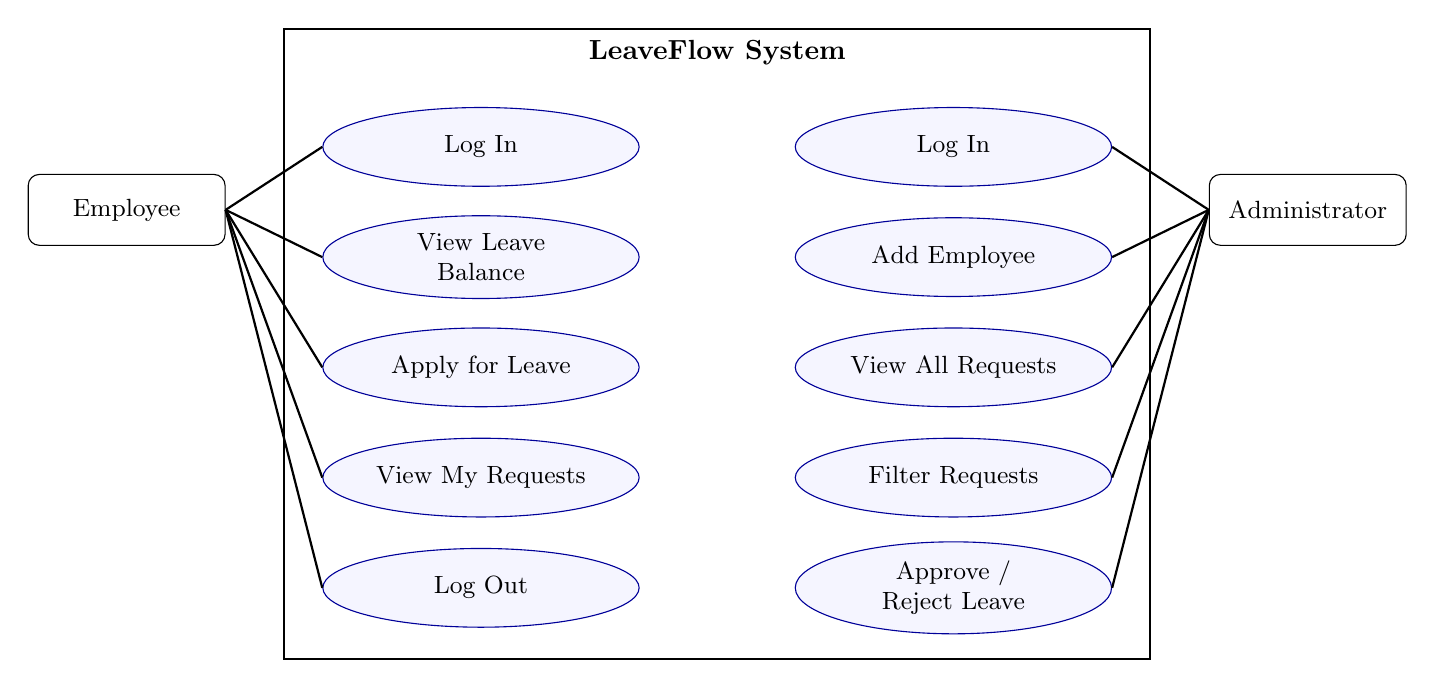
\begin{tikzpicture}[
    actor/.style={
        draw,
        rounded corners,
        align=center,
        minimum width=2.5cm,
        minimum height=0.9cm,
        font=\small
    },
    usecase/.style={
        draw=blue!60!black,
        fill=blue!4,
        ellipse,
        align=center,
        minimum width=3.2cm,
        text width=2.7cm,
        minimum height=1cm,
        inner sep=2pt,
        font=\small
    },
    link/.style={draw,thick}
]
% System boundary
\draw[thick] (0,0) rectangle (11,8);
\node[font=\bfseries] at (5.5,7.7) {LeaveFlow System};
% Actors
\node[actor] (employee) at (-2,5.7) {Employee};
\node[actor] (admin) at (13,5.7) {Administrator};
% Employee use cases
\node[usecase] (loginE) at (2.5,6.5) {Log In};
\node[usecase] (balance) at (2.5,5.1) {View Leave Balance};
\node[usecase] (apply) at (2.5,3.7) {Apply for Leave};
\node[usecase] (myrequests) at (2.5,2.3) {View My Requests};
\node[usecase] (logoutE) at (2.5,0.9) {Log Out};
% Administrator use cases
\node[usecase] (loginA) at (8.5,6.5) {Log In};
\node[usecase] (addemp) at (8.5,5.1) {Add Employee};
\node[usecase] (viewall) at (8.5,3.7) {View All Requests};
\node[usecase] (filter) at (8.5,2.3) {Filter Requests};
\node[usecase] (decision) at (8.5,0.9) {Approve / Reject Leave};
% Employee links
\draw[link] (employee.east) -- (loginE.west);
\draw[link] (employee.east) -- (balance.west);
\draw[link] (employee.east) -- (apply.west);
\draw[link] (employee.east) -- (myrequests.west);
\draw[link] (employee.east) -- (logoutE.west);
% Administrator links
\draw[link] (admin.west) -- (loginA.east);
\draw[link] (admin.west) -- (addemp.east);
\draw[link] (admin.west) -- (viewall.east);
\draw[link] (admin.west) -- (filter.east);
\draw[link] (admin.west) -- (decision.east);
\end{tikzpicture}%

}

\caption{Use-case diagram of the LeaveFlow system}

\label{fig:use-case}

\end{figure}



\section{Sequence Diagram}



The sequence diagram illustrates the flow of a leave application

from the employee to the backend components. The employee submits

the application through the web interface. Flask validates the

request fields and invokes the C++ executable to validate the dates,

calculate the duration, and check the maximum permitted leave

duration. If validation succeeds, the C++ backend saves the request

with a pending status and returns the result to Flask, which

communicates the outcome to the browser.



\begin{figure}[htbp]

\centering

\resizebox{0.95\textwidth}{!}{%

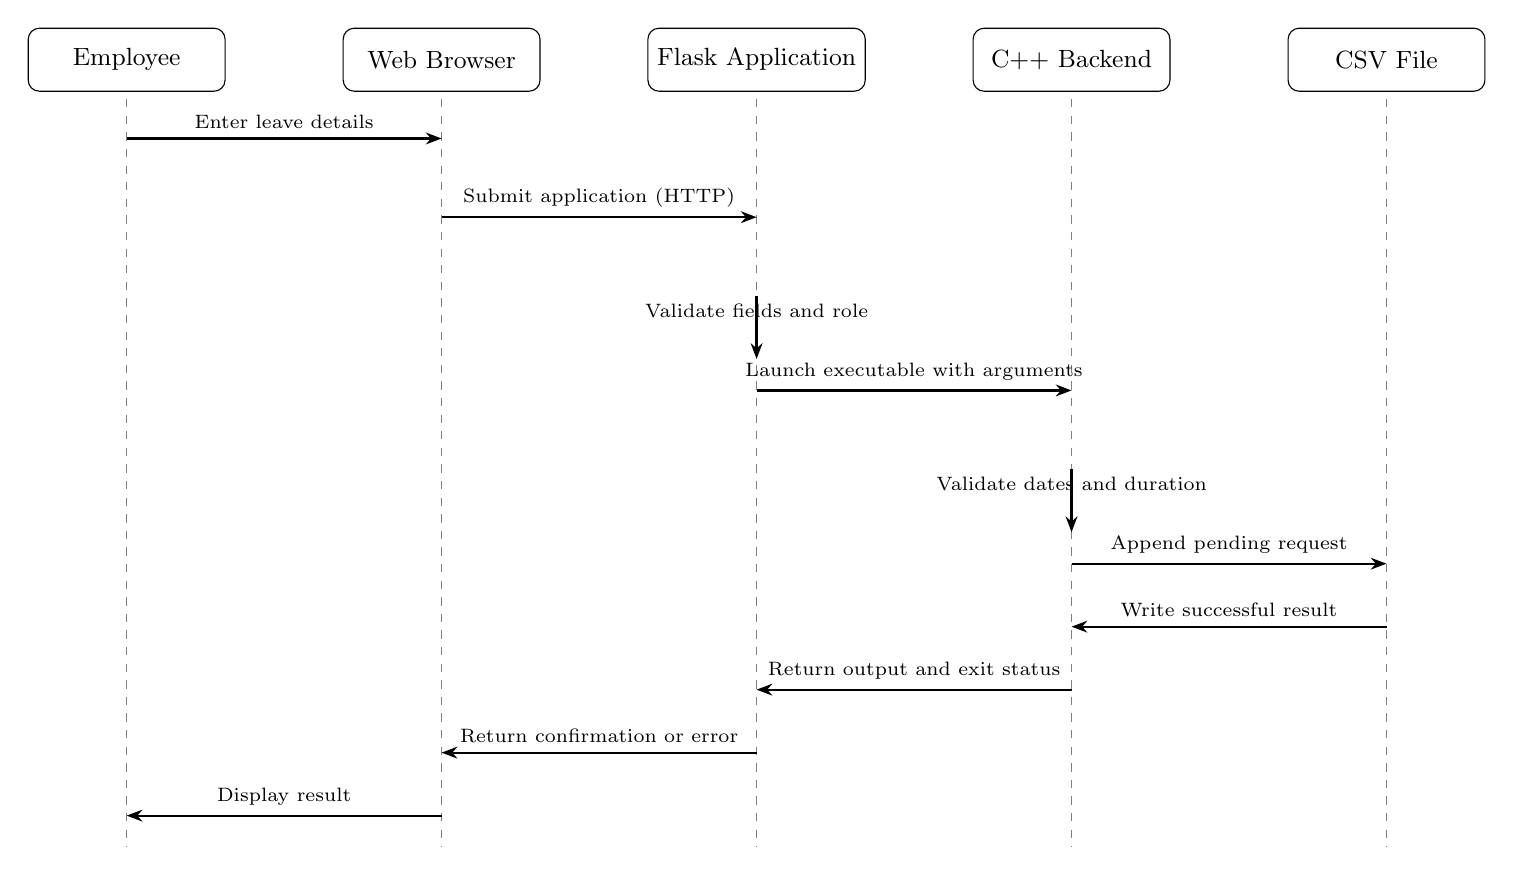
\begin{tikzpicture}[
    actor/.style={
        draw,
        rounded corners,
        align=center,
        minimum width=2.5cm,
        minimum height=0.8cm,
        font=\small
    },
    message/.style={-{Stealth[length=2mm]},thick},
    lifeline/.style={dashed,gray},
    every node/.style={font=\scriptsize}
]
% Participants
\node[actor] (employee) at (0,0) {Employee};
\node[actor] (browser) at (4,0) {Web Browser};
\node[actor] (flask) at (8,0) {Flask Application};
\node[actor] (cpp) at (12,0) {C++ Backend};
\node[actor] (csv) at (16,0) {CSV File};
% Lifelines
\foreach \x in {0,4,8,12,16} {
    \draw[lifeline] (\x,-0.5) -- (\x,-10);
}
% Messages
\draw[message] (0,-1) -- node[above] {Enter leave details} (4,-1);
\draw[message] (4,-2) -- node[above] {Submit application (HTTP)} (8,-2);
\draw[message] (8,-3) -- node[above] {Validate fields and role} (8,-3.8);
\draw[message] (8,-4.2) -- node[above] {Launch executable with arguments} (12,-4.2);
\draw[message] (12,-5.2) -- node[above] {Validate dates and duration} (12,-6);
\draw[message] (12,-6.4) -- node[above] {Append pending request} (16,-6.4);
\draw[message] (16,-7.2) -- node[above] {Write successful result} (12,-7.2);
\draw[message] (12,-8) -- node[above] {Return output and exit status} (8,-8);
\draw[message] (8,-8.8) -- node[above] {Return confirmation or error} (4,-8.8);
\draw[message] (4,-9.6) -- node[above] {Display result} (0,-9.6);
\end{tikzpicture}%

}

\caption{Sequence diagram for submitting a leave request}

\label{fig:leave-sequence}

\end{figure}



The activity diagram summarizes the administrator's decision process after a leave request is submitted. The administrator reviews a pending request and either rejects it or attempts to approve it. Approval depends on the employee having sufficient leave balance; if the balance is insufficient, the request remains pending. This workflow distinguishes a rejected request from an approved request and shows why a balance check is required before deducting leave.



\begin{figure}[htbp]

\centering

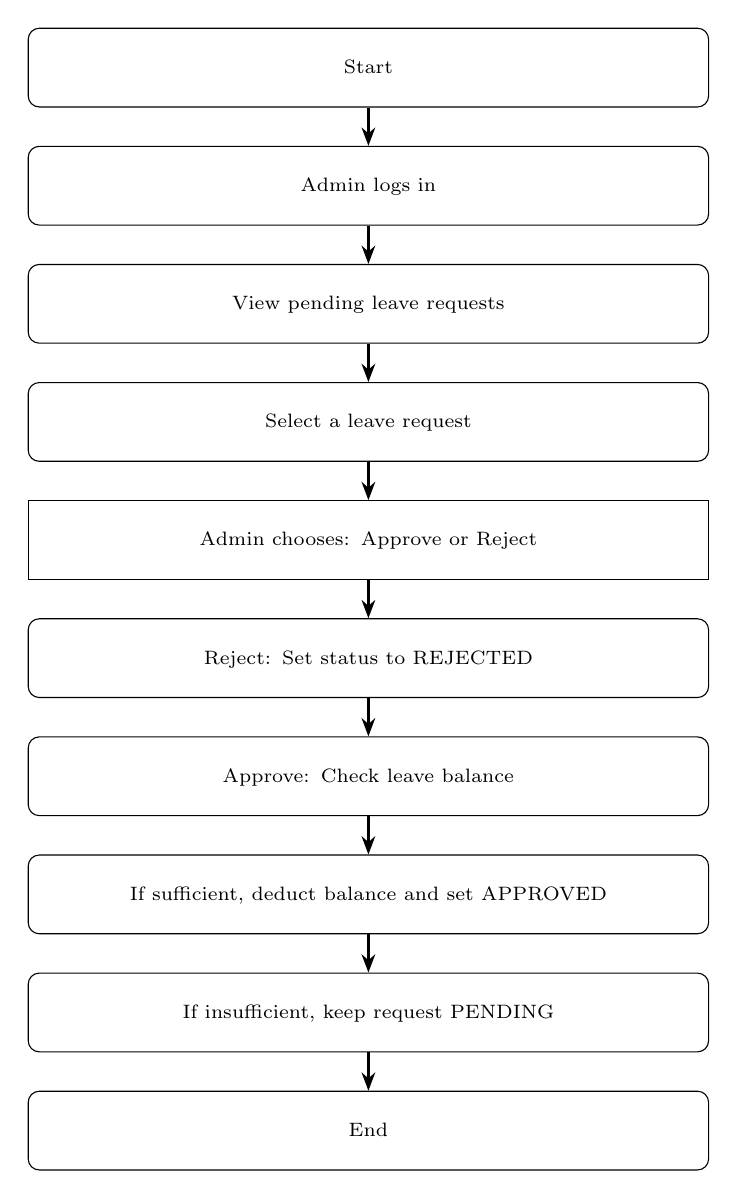
\begin{tikzpicture}[
    every node/.style={font=\scriptsize},
    box/.style={
        rectangle, draw, rounded corners,
        text width=8.5cm, minimum height=1.0cm,
        align=center, inner sep=2pt,
        text height=1.5ex, text depth=0.5ex
    },
    decision/.style={
        rectangle, draw,
        text width=8.5cm, minimum height=1.0cm,
        align=center, inner sep=2pt,
        text height=1.5ex, text depth=0.5ex
    },
    arrow/.style={->, >=Stealth, thick}
]
\node[box] (start) at (0,0) {Start};
\node[box] (login) at (0,-1.5) {Admin logs in};
\node[box] (view) at (0,-3.0) {View pending leave requests};
\node[box] (select) at (0,-4.5) {Select a leave request};
\node[decision] (check) at (0,-6.0) {Admin chooses: Approve or Reject};
\node[box] (reject) at (0,-7.5) {Reject: Set status to REJECTED};
\node[box] (balance) at (0,-9.0) {Approve: Check leave balance};
\node[box] (deduct) at (0,-10.5) {If sufficient, deduct balance and set APPROVED};
\node[box] (pending) at (0,-12.0) {If insufficient, keep request PENDING};
\node[box] (end) at (0,-13.5) {End};

% Equal-length vertical connectors between identically sized boxes
\draw[arrow] (start.south) -- (login.north);
\draw[arrow] (login.south) -- (view.north);
\draw[arrow] (view.south) -- (select.north);
\draw[arrow] (select.south) -- (check.north);
\draw[arrow] (check.south) -- (reject.north);
\draw[arrow] (reject.south) -- (balance.north);
\draw[arrow] (balance.south) -- (deduct.north);
\draw[arrow] (deduct.south) -- (pending.north);
\draw[arrow] (pending.south) -- (end.north);
\end{tikzpicture}

\caption{Activity diagram for leave request processing}

\label{fig:activity-diagram}

\end{figure}



The class diagram presents the main object-oriented components used in LeaveFlow. The abstract \texttt{User} class represents shared user details and operations, while \texttt{Employee} and \texttt{Admin} provide role-specific behaviour. The \texttt{LeaveBalance} class manages the available leave categories. The abstract \texttt{Leave} class defines common leave operations, and \texttt{CasualLeave}, \texttt{SickLeave}, and \texttt{EarnedLeave} provide leave-type-specific behaviour, including maximum duration limits.



\begin{figure}[htbp]

\centering

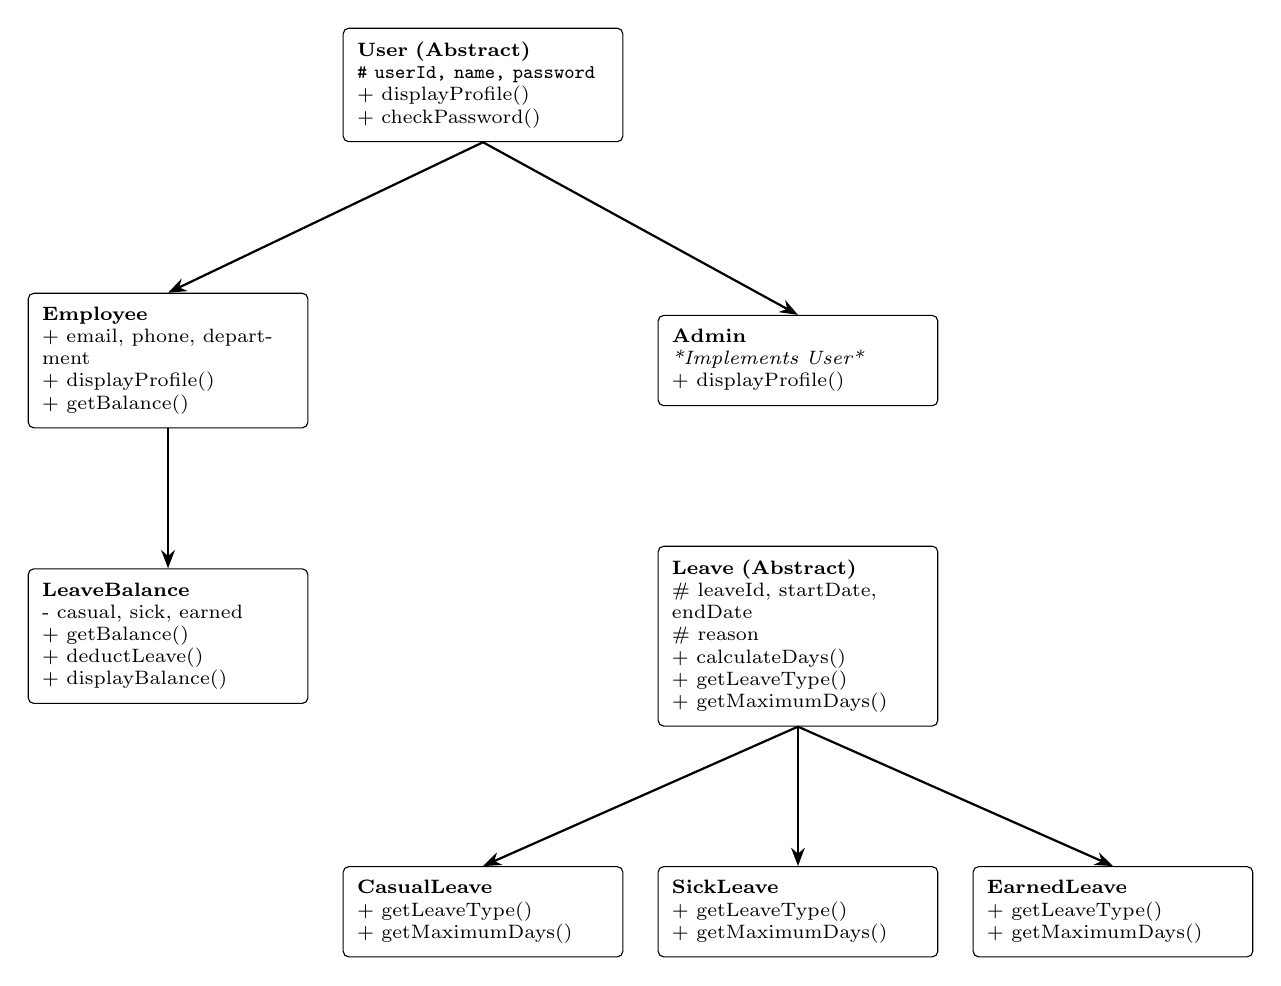
\begin{tikzpicture}[
    every node/.style={font=\scriptsize},
    class/.style={
        rectangle, draw, rounded corners=2pt,
        text width=3.2cm, align=left,
        inner sep=5pt
    },
    arrow/.style={-{Stealth}, thick}
]
\node[class] (user) at (0,0) {
    \textbf{User (Abstract)}\\
    
    \texttt{\# userId, name, password}\\
    
    + displayProfile()\\
    + checkPassword()
};
\node[class] (employee) at (-4,-3.5) {
    \textbf{Employee}\\
    
    + email, phone, department\\
    + displayProfile()\\
    + getBalance()
};
\node[class] (admin) at (4,-3.5) {
    \textbf{Admin}\\
    
    \textit{*Implements User*}\\
    + displayProfile()
};
\node[class] (balance) at (-4,-7) {
    \textbf{LeaveBalance}\\
    
    - casual, sick, earned\\
    
    + getBalance()\\
    + deductLeave()\\
    + displayBalance()
};
\node[class] (leave) at (4,-7) {
    \textbf{Leave (Abstract)}\\
    
    \# leaveId, startDate, endDate\\
    \# reason\\
    
    + calculateDays()\\
    + getLeaveType()\\
    + getMaximumDays()
};
\node[class] (casual) at (0,-10.5) {
    \textbf{CasualLeave}\\
    
    + getLeaveType()\\
    + getMaximumDays()
};
\node[class] (sick) at (4,-10.5) {
    \textbf{SickLeave}\\
    
    + getLeaveType()\\
    + getMaximumDays()
};
\node[class] (earned) at (8,-10.5) {
    \textbf{EarnedLeave}\\
    
    + getLeaveType()\\
    + getMaximumDays()
};
\draw[arrow] (user.south) -- (employee.north);
\draw[arrow] (user.south) -- (admin.north);
\draw[arrow] (employee.south) -- (balance.north);
\draw[arrow] (leave.south) -- (casual.north);
\draw[arrow] (leave.south) -- (sick.north);
\draw[arrow] (leave.south) -- (earned.north);
\end{tikzpicture}

\caption{Class diagram showing the main C++ classes in LeaveFlow}

\label{fig:class-diagram}

\end{figure}



\section{Implementation Procedure}



\subsection{Frontend Design}



The frontend of LeaveFlow provides a user-friendly web interface for employees and administrators. It is developed using HTML and CSS, with JavaScript used where required for user interactions. The interface includes a login page, an employee dashboard, a leave application form, and an administrative dashboard.



The login page allows users to enter their credentials and select their role. After successful authentication, employees can view their leave balances, submit leave requests, and track their request status. Administrators can access employee management and leave request review features.



The frontend communicates with the Flask application, which processes user requests and connects the interface to the backend logic and data storage.



\begin{figure}[htbp]

\centering

\IfFileExists{screenshots/login.png}{\IfFileExists{screenshots/login.png}{\includegraphics[width=0.8\textwidth]{screenshots/login.png}}{\fbox{\parbox{0.75\textwidth}{\centering Screenshot not supplied: \texttt{screenshots/login.png}}}}}{\fbox{\parbox{0.75\textwidth}{\centering Screenshot placeholder: screenshots/login.png}}}

\caption{LeaveFlow login interface}

\label{fig:login-interface}

\end{figure}



\begin{figure}[htbp]

\centering

\IfFileExists{screenshots/employee_dashboard.png}{\includegraphics[width=0.9\textwidth]{screenshots/employee_dashboard.png}}{\fbox{\parbox{0.75\textwidth}{\centering Screenshot not supplied: \texttt{screenshots/employee\_dashboard.png}}}}

\caption{Employee dashboard displaying leave balances and request information}

\label{fig:employee-dashboard}

\end{figure}



\subsection{Login and Role-Based Security}



LeaveFlow provides a login interface for employees and administrators. Users enter their credentials and select their role. The Flask application validates the login details using the user information stored in \texttt{users.json}. After successful authentication, a session is established to maintain the user's login state.



Role-based access control restricts access to different features. Employees can submit leave requests, view their own requests, and check their leave balances. Administrators can view all leave requests, manage employee accounts, and approve or reject requests.



The application checks the user's session and role before allowing access to protected routes. This prevents employees from accessing administrator-only operations through restricted URLs.



\begin{figure}[htbp]

\centering

\IfFileExists{screenshots/login_security.png}{\includegraphics[width=0.65\textwidth]{screenshots/login_security.png}}{\fbox{\parbox{0.75\textwidth}{\centering Screenshot not supplied: \texttt{screenshots/login\_security.png}}}}

\caption{Login interface showing credential fields and role selection}

\label{fig:login-security}

\end{figure}



The following simplified Python example illustrates session-based access control:



\begin{lstlisting}[language=Python,caption={Session-based access control},label={code:example-1}]
from flask import session, redirect, url_for



@app.route('/requests')

def requests_page():

    if 'username' not in session:

        return redirect(url_for('login'))



    if session.get('role') != 'admin':

        return "Access denied", 403



    return render_template('requests.html')
\end{lstlisting}



The session check ensures that the user is logged in, while the role check restricts the request-management page to administrators.

\subsection{Leave Request Submission}



Employees can submit leave requests by selecting the leave type, entering the start and end dates, and providing a reason. The Flask application receives the submitted details and invokes the C++ backend executable using Python's \texttt{subprocess} module.



The C++ backend validates the dates, calculates the leave duration, and checks the maximum permitted duration for the selected leave type. If the request is valid, it is stored in \texttt{leave\_requests.csv} with an initial status of \texttt{PENDING}. The result is returned to Flask, which displays a confirmation or error message to the employee.



\begin{figure}[htbp]

\centering

\IfFileExists{screenshots/leave_application.png}{\includegraphics[width=0.85\textwidth]{screenshots/leave_application.png}}{\fbox{\parbox{0.75\textwidth}{\centering Screenshot not supplied: \texttt{screenshots/leave\_application.png}}}}

\caption{Leave application form used by employees}

\label{fig:leave-application}

\end{figure}



The following simplified Python example illustrates how Flask invokes the C++ backend:



\begin{lstlisting}[language=Python,caption={Invoking the C++ backend using subprocess},label={code:example-2}]
import subprocess



result = subprocess.run(

    ["backend/leave_backend.exe",

     employee_id, leave_type,

     start_date, end_date, reason],

    capture_output=True,

    text=True

)
\end{lstlisting}



The backend's output and exit status are used by the Flask application to determine whether the request was processed successfully. This integration combines the web interface with the C++ leave-validation logic.



\subsection{Admin Approval, Rejection, and Leave-Balance Updates}



The administrator reviews pending leave requests through the admin dashboard. Each request displays the employee ID, leave type, dates, duration, reason, and current status. The administrator can approve or reject a request using the available controls.



When a request is approved, the Flask application verifies the employee's available leave balance. If sufficient balance is available, the requested number of days is deducted and the request status is changed to \texttt{APPROVED}. If the administrator rejects the request, its status becomes \texttt{REJECTED}, and the employee's balance remains unchanged.



The updated request status is displayed in the employee's request history. This allows employees to track the outcome of their applications. Keeping approval and rejection actions in the administrator interface also gives the workflow a clear separation of responsibilities: employees submit requests, while administrators review them. The balance is deducted only when a request is approved and the available balance is sufficient.



\begin{figure}[H]

\centering

\IfFileExists{screenshots/pending_requests.png}{\includegraphics[width=0.9\textwidth]{screenshots/pending_requests.png}}{\fbox{\parbox{0.75\textwidth}{\centering Screenshot not supplied: \texttt{screenshots/pending\_requests.png}}}}

\caption{Administrator interface for approving or rejecting pending leave requests}

\label{fig:admin-review}

\end{figure}



\begin{figure}[H]

\centering

\IfFileExists{screenshots/approval_confirmation.png}{\includegraphics[width=0.75\textwidth]{screenshots/approval_confirmation.png}}{\fbox{\parbox{0.75\textwidth}{\centering Screenshot not supplied: \texttt{screenshots/approval\_confirmation.png}}}}

\caption{Successful leave request approval confirmation}

\label{fig:approval-success}

\end{figure}



\begin{figure}[H]

\centering

\IfFileExists{screenshots/request_history.png}{\includegraphics[width=0.85\textwidth]{screenshots/request_history.png}}{\fbox{\parbox{0.75\textwidth}{\centering Screenshot not supplied: \texttt{screenshots/request\_history.png}}}}

\caption{Employee request history displaying approved and rejected requests}

\label{fig:updated-request-status}

\end{figure}



\begin{figure}[H]

\centering

\IfFileExists{screenshots/updated_balances.png}{\includegraphics[width=0.9\textwidth]{screenshots/updated_balances.png}}{\fbox{\parbox{0.75\textwidth}{\centering Screenshot not supplied: \texttt{screenshots/updated\_balances.png}}}}

\caption{Updated leave balances after approval of a leave request}

\label{fig:balance-update}

\end{figure}



\subsection{Data Storage and Management}



LeaveFlow uses JSON and CSV files for persistent local data storage. These files maintain employee information, leave balances, and leave request records.



\begin{itemize}

    \item \textbf{users.json:} Stores employee account information used by the Flask application during authentication.



    \item \textbf{leave\_balances.json:} Stores the available casual, sick, and earned leave balances for employees. The application updates these balances when leave requests are approved.



    \item \textbf{leave\_requests.csv:} Stores submitted leave requests, including employee ID, leave type, start date, end date, duration, reason, and request status.

\end{itemize}



The Flask application reads and updates these files to display request histories, manage employee balances, and process administrative decisions. The C++ backend appends valid leave requests to the CSV file with an initial status of \texttt{PENDING}.



During approval or rejection, the application updates the relevant records. Temporary files are used before replacing the original files during updates, helping reduce the risk of partially written data.



This file-based approach is suitable for a small academic project because it is simple to implement and does not require a separate database server. Each file has a distinct responsibility: account data supports authentication, balance data supports leave availability checks, and request records preserve the history and current status of applications. Because these files are local, the application is best suited to a small demonstration or academic deployment rather than a high-concurrency production environment.



\begin{figure}[htbp]

\centering

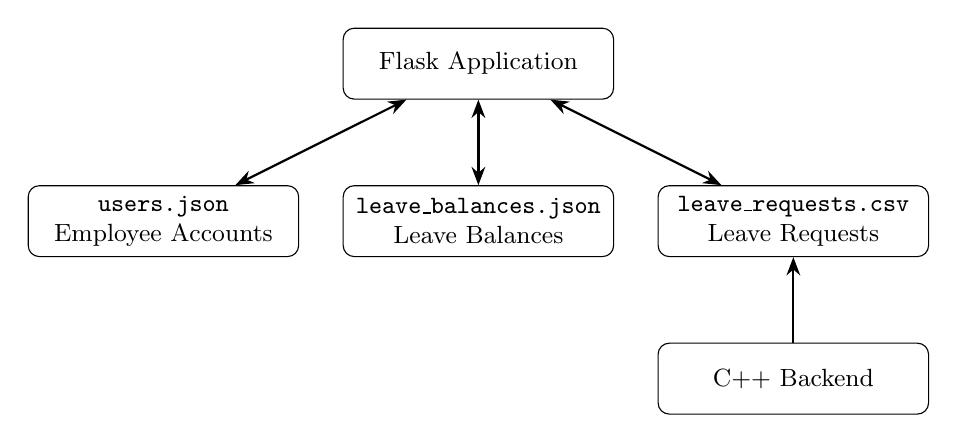
\begin{tikzpicture}[
    every node/.style={font=\small},
    component/.style={
        rectangle, draw, rounded corners,
        text width=3.2cm, minimum height=0.9cm,
        align=center
    },
    arrow/.style={->, >=Stealth, thick}
]
\node[component] (flask) at (0,0)
    {Flask Application};
\node[component] (users) at (-4,-2)
    {\texttt{users.json}\\Employee Accounts};
\node[component] (balances) at (0,-2)
    {\texttt{leave\_balances.json}\\Leave Balances};
\node[component] (requests) at (4,-2)
    {\texttt{leave\_requests.csv}\\Leave Requests};
\node[component] (cpp) at (4,-4)
    {C++ Backend};
\draw[arrow,<->] (flask) -- (users);
\draw[arrow,<->] (flask) -- (balances);
\draw[arrow,<->] (flask) -- (requests);
\draw[arrow] (cpp) -- (requests);
\end{tikzpicture}

\caption{Data storage and interaction between the application components}

\label{fig:data-storage}

\end{figure}



\FloatBarrier

\section{Testing and Results}



The LeaveFlow application was tested to verify its main features and the interaction between the frontend, Flask application, C++ backend, and local data files.



\begin{table}[H]

\centering

\renewcommand{\arraystretch}{1.2}

\begin{tabularx}{\textwidth}{|>{\centering\arraybackslash}p{1.1cm}|p{3.3cm}|X|}

\hline

\textbf{S.No.} & \textbf{Test Case} & \textbf{Expected Result} \\

\hline

1 & User login & The user accesses the appropriate interface after successful authentication. \\

\hline

2 & Submit leave request & A valid request is stored with \texttt{PENDING} status. \\

\hline

3 & Approve leave request & The status changes to \texttt{APPROVED}, and the available leave balance is reduced. \\

\hline

4 & Reject leave request & The status changes to \texttt{REJECTED} without deducting leave. \\

\hline

5 & View request history & The employee can view the status of their submitted requests. \\

\hline

6 & Role-based access & Administrative operations are restricted to authorized administrators. \\

\hline

7 & View leave balance & The employee can view updated casual, sick, and earned leave balances. \\

\hline

\end{tabularx}

\caption{Functional testing of LeaveFlow}
\label{tab:functional-testing}

\end{table}



The screenshots demonstrate the application's login interface, pending requests, approval confirmation, request history, and updated leave balances. In the demonstrated two-day sick-leave approval, the available sick-leave balance decreased from 10 days to 8 days.



The results show that the major application workflows operate across the web interface, Flask application, C++ backend, and local data files. The test cases cover successful actions, such as login and approval, as well as access and status checks, such as role restrictions and rejection without balance deduction. Together, these checks provide evidence that the main employee and administrator workflows are connected end to end.



\section{Additional Features}



\subsection{Employee Account Creation}



LeaveFlow allows administrators to create employee accounts through the employee management interface. The administrator enters the employee's name and a temporary password. The application creates the account and initializes the default casual, sick, and earned leave balances. This feature simplifies employee onboarding.



\begin{figure}[htbp]

\centering

\IfFileExists{screenshots/add_employee.png}{\includegraphics[width=0.9\textwidth]{screenshots/add_employee.png}}{\fbox{\parbox{0.75\textwidth}{\centering Screenshot not supplied: \texttt{screenshots/add\_employee.png}}}}

\caption{Interface for adding a new employee}

\label{fig:add-employee}

\end{figure}



\subsection{Leave Request Filtering}



Administrators can filter leave requests by status, including All Requests, Pending, Approved, and Rejected. This makes it easier to find requests that need attention and review previously processed applications.



\begin{figure}[htbp]

\centering

\IfFileExists{screenshots/request_filter.png}{\includegraphics[width=0.9\textwidth]{screenshots/request_filter.png}}{\fbox{\parbox{0.75\textwidth}{\centering Screenshot not supplied: \texttt{screenshots/request\_filter.png}}}}

\caption{Filtering leave requests by status}

\label{fig:request-filter}

\end{figure}



\subsection{Administrative Summary Dashboard}



The administrative dashboard summarizes leave activity, including the total number of requests and the numbers of approved and rejected applications. It also displays pending requests, helping the administrator quickly understand the current state of leave processing.



\begin{figure}[htbp]

\centering

\IfFileExists{screenshots/admin_summary.png}{\includegraphics[width=0.95\textwidth]{screenshots/admin_summary.png}}{\fbox{\parbox{0.75\textwidth}{\centering Screenshot not supplied: \texttt{screenshots/admin\_summary.png}}}}

\caption{Administrative dashboard showing leave request statistics}

\label{fig:admin-summary}

\end{figure}



\subsection{C++ and Flask Integration}



Flask invokes the compiled C++ executable with the employee ID, leave type, start date, end date, and reason. The executable processes the arguments and returns output and an exit status. Flask uses this result to decide whether to display a success or error message to the employee. This integration allows the web interface and C++ validation logic to work together.



\begin{lstlisting}[language=Python,caption={Handling the C++ backend result},label={code:example-3}]
result = subprocess.run(

    ["backend/leave_backend.exe",

     employee_id, leave_type,

     start_date, end_date, reason],

    capture_output=True,

    text=True

)



if result.returncode == 0:

    message = result.stdout

else:

    message = result.stderr or result.stdout
\end{lstlisting}



The snippet is illustrative and should be checked against the actual Flask route before being described as an exact extract from the source code.



\subsection{Date and Leave-Duration Validation}



LeaveFlow incorporates date validation and leave-duration calculation in its C++ backend. The abstract \texttt{Leave} class defines the common structure and operations for different leave types. Its \texttt{calculateDays()} function parses the start and end dates using \texttt{std::get\_time()}, converts them into time values using \texttt{std::mktime()}, and calculates the difference between the dates.



The function returns zero if date parsing or time conversion fails. For valid conversions, it calculates the duration in days and adds one to include both the start and end dates.



\begin{lstlisting}[language=C++,caption={Leave duration calculation},label={code:example-4}]
int Leave::calculateDays() const {

    std::tm start = {};

    std::tm end = {};



    std::istringstream startInput(startDate);

    std::istringstream endInput(endDate);



    startInput >> std::get_time(&start, "%Y-%m-%d");

    endInput >> std::get_time(&end, "%Y-%m-%d");



    if (startInput.fail() || endInput.fail()) {

        return 0;

    }



    start.tm_isdst = -1;

    end.tm_isdst = -1;



    std::time_t startTime = std::mktime(&start);

    std::time_t endTime = std::mktime(&end);



    if (startTime == static_cast\<std::time_t>(-1) ||

        endTime == static_cast\<std::time_t>(-1)) {

        return 0;

    }



    double seconds = std::difftime(endTime, startTime);

    int days = static_cast\<int>(

        seconds / (60 \* 60 \* 24)

    );



    return days + 1;

}
\end{lstlisting}



The maximum permitted duration is defined separately for each leave type through polymorphism. For example, the \texttt{CasualLeave} class restricts casual leave to three days.



\begin{lstlisting}[language=C++,caption={Maximum permitted casual-leave duration},label={code:example-5}]
int CasualLeave::getMaximumDays() const {

    return 3;

}
\end{lstlisting}



\begin{figure}[H]

\centering

\IfFileExists{screenshots/date_parsing.png}{\includegraphics[width=0.9\textwidth]{screenshots/date_parsing.png}}{\fbox{\parbox{0.75\textwidth}{\centering Screenshot not supplied: \texttt{screenshots/date\_parsing.png}}}}

\caption{Date parsing and validation in the calculateDays() function}

\label{fig:date-parsing}

\end{figure}



\begin{figure}[H]

\centering

\IfFileExists{screenshots/duration_calculation.png}{\includegraphics[width=0.9\textwidth]{screenshots/duration_calculation.png}}{\fbox{\parbox{0.75\textwidth}{\centering Screenshot not supplied: \texttt{screenshots/duration\_calculation.png}}}}

\caption{Time conversion and leave-duration calculation in Leave.cpp}

\label{fig:duration-calculation}

\end{figure}



\begin{figure}[H]

\centering

\IfFileExists{screenshots/leave_base_class.png}{\includegraphics[width=0.85\textwidth]{screenshots/leave_base_class.png}}{\fbox{\parbox{0.75\textwidth}{\centering Screenshot not supplied: \texttt{screenshots/leave\_base\_class.png}}}}

\caption{Abstract Leave class with virtual functions}

\label{fig:leave-base-class}

\end{figure}



\begin{figure}[H]

\centering

\IfFileExists{screenshots/casual_leave_limit.png}{\includegraphics[width=0.85\textwidth]{screenshots/casual_leave_limit.png}}{\fbox{\parbox{0.75\textwidth}{\centering Screenshot not supplied: \texttt{screenshots/casual\_leave\_limit.png}}}}

\caption{CasualLeave class defining the maximum permitted duration}

\label{fig:casual-leave-limit}

\end{figure}



This design keeps the common date-calculation logic in the base class while allowing derived classes to specify their own leave-duration limits. The same approach can be used for sick leave and earned leave.



\FloatBarrier

\section{Conclusion}



LeaveFlow is a web-based Employee Leave Management System developed to simplify and streamline the leave application and approval process. It provides separate interfaces for employees and administrators, enabling employees to apply for leave, view their leave balances, and track request statuses, while administrators can manage employee accounts and process leave requests.



The system integrates HTML and CSS for the user interface, Flask for application logic, and C++ for leave validation and duration calculation. JSON and CSV files are used for data storage. The project demonstrates object-oriented programming concepts such as abstraction, inheritance, encapsulation, and polymorphism, along with integration between different programming technologies.



The successful implementation of the major workflows demonstrates how LeaveFlow can make leave management more organized, efficient, and transparent.



\end{document}